\documentclass[tikz,border=2pt]{standalone}
\usepackage{amsmath}
\usepackage{pgfplots}
\pgfplotsset{compat=1.18}

\begin{document}
% The roots of p(x) = (x+2)(x-1)(x-3)/4 are where its graph meets the x-axis; each root r
% gives a linear factor (x - r).
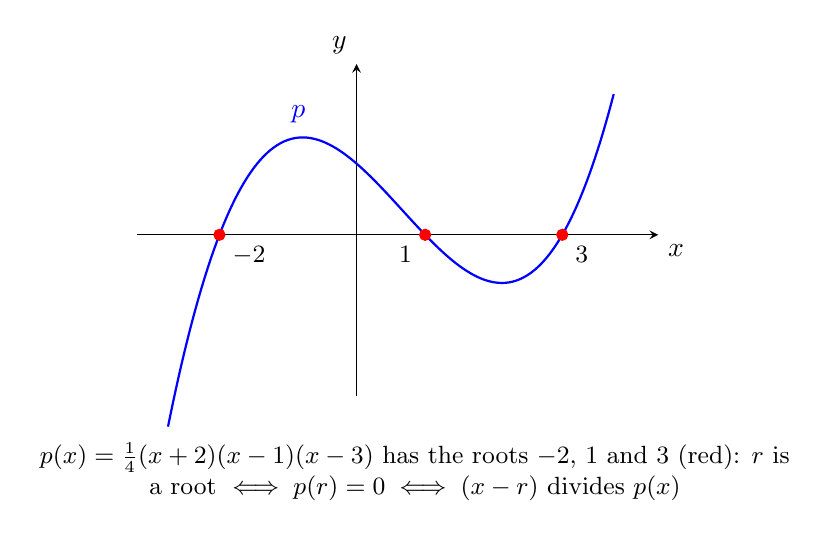
\begin{tikzpicture}
	\begin{axis}[
		axis lines=middle,
		xmin=-3.2, xmax=4.4, ymin=-3.4, ymax=3.6,
		xtick={-2,1,3}, xticklabels={,,}, ytick=\empty,
		xlabel={$x$}, ylabel={$y$},
		xlabel style={below right}, ylabel style={above left},
		samples=120, smooth, clip=false,
		width=8.2cm, height=5.8cm
		]
		\addplot[thick, blue, domain=-2.75:3.75] {(x+2)*(x-1)*(x-3)/4};
		\addplot[only marks, mark=*, red, mark size=2pt] coordinates {(-2,0) (1,0) (3,0)};
		\node[anchor=north west, font=\small] at (axis cs:-1.95,-0.05) {$-2$};
		\node[anchor=north east, font=\small] at (axis cs:0.95,-0.05) {$1$};
		\node[anchor=north west, font=\small] at (axis cs:3.05,-0.05) {$3$};
		\node[blue, anchor=south] at (axis cs:-0.85,2.15) {$p$};
	\end{axis}
	\node[anchor=north, font=\small, align=flush center, text width=9.6cm] at ([yshift=-2pt]current axis.outer south) {$p(x)=\tfrac14(x+2)(x-1)(x-3)$ has the roots $-2$, $1$ and $3$ (red): $r$ is a root $\iff p(r)=0\iff(x-r)$ divides $p(x)$};
\end{tikzpicture}
\end{document}
